\section{Numerical solution of The Non linear Shallow Water Equation}
 The one dimensional Non Linear Shallow Water Equations (NSWE) with flat bottom read in conservation form

\begin{equation}
	\begin{split}
		h_t + ( hu)_x = 0\\
		(hu)_t + \left( hu^2 + \frac{1}{2}gh^2 \right)_x = 0 
	\end{split}
	\label{serre:nswe}
\end{equation}

 where subscripts denote partial derivatives respect to time and space variables $t$ and $x$; $h$ denotes the water column height; $u$ the horizontal velocity; $g=9.81$ the gravity acceleration. As a conservation law, the system \eqref{serre:nswe} can be written as

\begin{equation}
	U_t + F(U)_x = 0
	\label{serre:conservative_swe}
\end{equation}

 where $U=(h,hu)^T$, $F(U) = (hu, hu^2 + \frac{1}{2}gh^2)$. Weak solutions are approximated using a Finite Volume scheme. After averaging the system \eqref{serre:conservative_swe} in a cell $\Omega_i = [x_i-\Delta x/2, x_i+\Delta x/2]$, and defining $ \overline U = \frac{1}{\Delta x} \int_{\Omega_i} U(x)dx$, then a semidiscrete approximation to \eqref{serre:conservative_swe} is 

\begin{equation}
	\overline U _t + \frac{1}{\Delta x}\left( F(U_{i+1/2}) - F(U_{i-1/2}) \right) = 0
	\label{serre:semidiscrete_swe}
\end{equation}

 where $U_{i\pm1/2}$ corresponds to the values of the conserved variables at the interface of each cell. The system \eqref{serre:semidiscrete_swe} is integrated in time using an Euler scheme with CFL condition

\begin{equation}
	\Delta t = CFL \frac{\Delta x}{\max_i(|u_i|+c_i)}
\end{equation}

with $CFL=0.45$.

\subsection{Riemann problem}
At each time-step the the values at each interface $U^* = U_{i+1/2}$ of system \eqref{serre:semidiscrete_swe} are obtained from the solution to the Riemann problem of the non-conservative form of \eqref{serre:conservative_swe} between the two neighbor states $U_L = U_i$ and $U_R = U_{i+1}$

\begin{equation}
	\begin{split}
	  U_t + A(U) U_x = 0 \\
	  U(t=0,x) = \begin{cases}
		 U_l &, \text{ if } x\leq 0. \\
		 U_r &, \text{ if } x > 0 
		\end{cases}
	\end{split}
	\label{serre:nonconservative_swe_1}
\end{equation}

 where $A$ is the jacobian matrix of $F(U)$. The solution to this Riemann problem is found using the approximate Riemann solver of Roe that is described in reference \cite{marche2006}. It consists first of a change of variables that allows to write \eqref{serre:nonconservative_swe_1} for $h>0$ as

\begin{equation}
	\begin{split}
	  V_t + C(V)V_x = 0 \\
	  V(t=0,x) = \begin{cases}
		V_l &, \text{ if } x\leq 0. \\
	 V_r &, \text{ if } x > 0 
		\end{cases}
	\end{split}
	\label{serre:nonconservative_swe_2}
\end{equation}

 with $V = (2c,u)^T$ and 
$C(V) = \left( 
\begin{array}{cc} 
u & c \\ 
c & u \end{array}\right)$. Second, instead of using the exact formulation, a linearized problem is solved using $C(\hat V)$ in place of $C(V)$, with $\hat V = (V_L +V_R)/2$. The matrix $C(\hat V)$ is diagonalizable and thus, a decoupled system can be obtained in the form

\begin{equation}
	\begin{split}
		(w_1)_t + \hat \lambda_1 (w_1)_x = 0\\
		(w_2)_t + \hat \lambda_2 (w_2)_x = 0 \\	
	(w_1,w_2)^T(t=0,x) = \begin{cases}
		((w_1)_L,(w_2)_L)^T &, \text{ if } x\leq 0. \\
		((w_1)_L,(w_2)_L)^T &, \text{ if } x > 0 
		\end{cases}
	\end{split}
\end{equation}

 where $\hat \lambda_1 = \hat u - \hat c$, $\hat \lambda_2 = \hat u + \hat c$, $w_1 = u-2c$, $w_2 = u+2c$ and $ (w_1)_L = u_L - 2c_L, (w_2)_L = u_L - 2c_L$, $ (w_1)_R = u_R - 2c_R, (w_2)_R = u_R - 2c_R$. Writing $W=(w_1,w_2)$ and noticing that $\hat \lambda_1 \leq \hat \lambda_2$, the solution can be found for three separate cases:

\begin{itemize}
	\item If $\lambda_1 > 0$, then $W^* = W_L$
	\item If $\lambda_1 \leq 0 $ and $\lambda_2>0$, $W^* = ((w_R)_1, (w_L)_2)^T$
	\item If $\lambda_2\leq 0 $, $W^* = W_R$
\end{itemize}

 and values at the interface can then be recovered setting the inverse transformation 

\begin{equation}
	\begin{split}
	u^* = \frac{1}{2}(w^*_1+w^*_2) \\
	h^* = \frac{1}{16g}(w^*_2-w^*_1)^2
	\end{split}	
	\label{serre:riemman_solution}
\end{equation}

A third step is necessary, which consists on an entropy fix to select only weak solutions that are physically consistent. This is simply obtained by setting $W^* = \hat W$ whenever $(\lambda_1)_L < 0$ and $(\lambda_1)_r >0$, or $(\lambda_2)_L < 0 $ and $(\lambda_2)_R>0$.

\subsection{Second order MUSCL Scheme}

To obtain second order convergence for smooth solutions a MUSCL (Monotonic Upstream-Centered) scheme is used. This means that instead of solving a Riemann problem between $U_L=U_{i}$ and $U_R=U_{i+1}$ one must solve for 
$U_L = U_{i,r}$ and $U_R=U_{i+1,l}$, 
where $U_{i,r} = U_i + \frac{\Delta x}{2} s$, 
$U_{i,l} = U_i - \frac{\Delta x}{2} s$  $s = minmod(s_L,s_R)$, 
$s_L = \frac{U_{i}-U_{i-1}}{\Delta x}$, 
$s_R = \frac{U_{i+1}-U_{i}}{\Delta x}$ and

\begin{equation}
	minmod(s_1,s_2) = \begin{cases}
		min(s_1,s_2) & \text{ if } s_1>0 \textit{ and } s_2>0 \\
		max(s_1,s_2) & \text{ if } s_1<0 \textit{ and } s_2<0 \\
		0 & elsewhere
	\end{cases}
\end{equation}

\subsection{Fourth order MUSCL scheme}

In order to decrease the truncation dispersion and dissipation error a fourth order MUSCL scheme is also used, using the methodology explained in \cite{Bonneton2011}. The MUSCL scheme proposes to reconstruct values at the interface comparing three different slopes which will serve to interpolate the cells values up to the interface. First we compute the difference values $\delta h_{i,l}$ and $\delta h_{i,r}$ given by equations \eqref{serre:muscl4_dhil} and \eqref{serre:muscl4_dhir}

\begin{dmath}
    \delta h_{i,l} = 
    (1-\nu)(h_i^n-h_{i-1}^n) + 
    \nu(h_{i+1}^n-h_{i}) +
    \xi^c(-h_{i-2}+3h_{i-1}^n-3h_i^n+h_{i+1}^n) +
    \xi^d(-h_{i-1}^n +3h_i^n - 3h_{i+1}^n+h_{i+2}^n )
\label{serre:muscl4_dhil}
\end{dmath}

\begin{dmath}
        \delta h_{i,r} = 
        (1-\nu)(h_{i+1}^n-h_i^n) + 
        \nu( h_i^n - h_{i-1}) + 
        \xi^c( -h_{i-1}^n + 3h_i^n - 3h_{i+1}^n + h_{i+2}^n) +
        \xi^d(-h_{i-2}^n + 3h_{i-1} -3 h_i^n + h_{i+1}^n) 
        \label{serre:muscl4_dhir}
\end{dmath}

 which are to be compared with the forward and backward differences $ \delta h_i^{n,+} = h_{i+1}^n-h_i^n$ and $ \delta h_i^{n,-} = h_i^n - h_{i-1}^n$. Values of $\nu, \xi^c$ and $\xi^d$ of $\frac{1}{3}$, $-\frac{1}{10}$ and $-\frac{1}{15}$ were chosen, as proposed in \cite{Bonneton2011}, which have the best numerical dissipation and dispersion error.

Second, limited values are obtained at the left and right boundary of each cell according to the formula

\begin{equation}
\begin{split}
    ^Lh_{i,l}^n = h_i^n -\frac{1}{2} L_{i,l}(h^n) & \text{ for } i=0 ..n_x \\
    ^Lh_{i,r}^n = h_i^n + \frac{1}{2} L_{i,r}(h^n) & \text{ for } i=-1...n_x-1     
\end{split}
\end{equation}

 where $L_{i,r}(h^n) = L (\delta h_i^{n,-}, \delta h_i^{n,+}, \delta h_{i,r}^n)$,
$L_{i,l}(h^n) = L (\delta h_i^{n,+}, \delta h_i^{n,-}, \delta h_{i,l}^n)$, and
\begin{equation}
    L(u,v,w) = \begin{cases}
        0 & \text{ if } uv\leq 0 \\
        sign(u)\min(2|u|,2|v|,w) & \text{ if } uv>0
    \end{cases}
\end{equation}


 The reconstruction proposes to apply this procedure to both $h_i$ and $(hu)_i$ to obtain reconstructed states $^LU_{i,r}$ and $^LU_{i,l}$, and then calculate the values $U_{i+1/2}$ at each interface by solving the Riemann problem between states $U_L=^LU_{i,r}$ and $U_R = ^LU_{i+1,l}$.

\subsection{Boundary conditions}
\label{nswe:bcs}

Homogeneous Neumann or Dirichlet boundary conditions are considered, which imply the use of additional ghost cells whose number depends on each particular scheme. Considering a 0-based index for the domain, i.e, the domain interior is defined for $x_i$ with $i$ from $0$ to $n_x-1$, for any quantity $\phi_i$ boundary conditions are defined as follows,

\begin{itemize}
	\item Homogeneous Neumann (HN): \begin{equation}
		\begin{split}
			\phi_{-i} = \phi_{i-1} \\
			\phi_{n_x-1+i} = \phi_{n_x-i}
		\end{split}
		\label{nswe:neumann}
	\end{equation}
	for $i$ from $1$ to $k$

	\item Homogeneous Dirichlet (HD): \begin{equation}
		\begin{split}
			\phi_{-i} = -\phi_{i-1} \\
			\phi_{n_x-1+i} = -\phi_{n_x-i}
		\end{split}
	\end{equation}
\end{itemize}

With $k=1, 2, 3$ for the first, second and fourth order scheme respectively. Open boundaries are defined then as HN for $h$ and $hu$, and closed boundaries as HN for $h$ and HD for $hu$.

\section{Verification}

Two analytical solutions to the NSWE are used to test the implementation of the three schemes explained. Both solutions correspond to the idealized one-dimensional representation of a dam break over a horizontal channel with dry or wet bottom, respectively. 

The analytical solution for the case with wet bottom is

\begin{equation}
	h(t,x) = \begin{cases}
		h_l & x\leq x_a(t) \\
		\frac{4}{9g}\left(\sqrt{gh_L}- \frac{x-x_0}{2t} \right)^2 & x_a(t) < x \leq x_b(t) \\
		\frac{c_m^2}{2g} & x_b(t) < x \leq x_c(t) \\
		h_r & x_c(t) < x
	\end{cases}
\end{equation}

\begin{equation}
	u(t,x) = \begin{cases}
		0 & x \leq x_a(t)\\
		\frac{2}{3}\left( \frac{x-x_0}{t} + \sqrt{gh_L} \right) & x_a(t) < x \leq x_b(t) \\
		2(\sqrt{gh_L}-c_m) & x_b(t) < x \leq x_c(t) \\
		0 & x_c(t) < x
	\end{cases}
\end{equation}

 where $h_l$ is the water height at the reservoir located initially at $x\leq 0$ and $x_a(t)= -t\sqrt{gh}$, $x_b(t) = t(2\sqrt{gh_l} - 3c_m$, $x_c(t) = x_0 + t 2cm^2 \frac{\sqrt{gh_l}-c_m}{c_m^2-gh_r}$ and $c_m$ is the solution to the non-linear equation $$-8gh_rc_m^2(\sqrt{gh_l}-c_m)^2 + (c_m^2-gh_r)^2(c_m^2+gh_r)=0$$
 whose solution is obtained numerically up to machine precision. 

The analytical solution for the case with dry bottom is

\begin{equation}
	h(t,x) = \begin{cases}
		h_l, &\text{ if }x \leq x_a(t)\\
		\frac{4}{9g}\left(c_l - \frac{x-x_0}{2t}\right), &\text{ if }x_a(t)<x\leq x_b(t) \\
		0, &\text{ if } x_b(t)\leq x
	\end{cases}	
\end{equation}

where $x_a(t) = - t\sqrt{gh_l}$ and $x_b(t) = 2t \sqrt{gh_l}$

\subsection{Results}

	Simulations were tested for different configurations on both cases considering a wet or dry channel as initial condition. For all cases the water in the reservoir starts at rest with a height of $10m$, and $1m$ in the channel for the wet-case. The domain is the interval $[-L,L]$ with $L=30$, with the reservoir in the region $x<0$ and the discretization considers a space step of $\Delta x = 	30/100$ and $CFL=0.45$. Different configurations were tested considering open or closed boundary conditions for the three schemes.

	\subsubsection{First order scheme}

	Table \ref{nswe:dbresults} summarizes results for eight different cases studied in the first order scheme model. For Case 1, with an initially wet-channel, reasonable agreement is found with respect to the analytical solution as can be seen in figures \ref{nswe:wetchannel} for both open and closed boundaries. However, when imposing an initially dry case and closed boundaries in Case 2, negative water heights are observed, which, as was seen in the simulations, originate from the right boundary once the wave reaches that point. This kind of error is not observed for Case 3 which only differs on the use of Open Boundary conditions.

	To see if this error was by coincidence an issue with the boundary at $x=L$ the same simulation as Case 2 was performed but using the interval $[-2L,2L$ as domain in Case 4. It was verified that the error appears not at $x=L$ now but at the right boundary $x=2L$.

	Also, to test the sensitivity to a 0 water height on the downstream channel, a small values was set at the beginning of the simulation. Values of $10^{-4}m$ for cases 5 and $10^{-5}m$ for cases 6 and 7 were set. It was observed that, when using closed boundaries, Case 5 did not show negative depth heights, but interaction with the boundary caused an abnormal higher water depth and an increased oscillation, as can be seen in figure \ref{nswe:drychannel}. In Case 6 however negative depths were observed, which were absent when changing to open boundary conditions.

	Finally, Case 8 shows results obtained for the dambreak case with dry channel, but using the SurfWB-UC model developed in reference \cite{guerra2014}. It was confirmed that indeed the closed boundary condition causes trouble in the simulation, as can be seen in figure \ref{nswe:surfwb}.

	\begin{table}[]
	\centering
	\label{my-label}
	\begin{tabular}{|l|l|l|l|}
	\hline
	\textbf{Case \#} & \textbf{IC}    & \textbf{BC} & \textbf{Status}                  \\ \hline
	1                & Wet            & Closed/Open & $\checkmark$                       \\ \hline
	2                & Dry            & Closed      & $\times$                             \\ \hline
	3                & Dry            & Open        & $\checkmark$                       \\ \hline
	4                & Dry $[-2L,2L]$ & Open        & $\checkmark$ at $(x=L)$, $\times$ at $x=2L$ \\ \hline
	5                & Dry $10^{-4}$  & Closed      & $\checkmark$                          \\ \hline
	6                & Dry $10^{-5}$  & Closed      & $\times$                   		\\ \hline
	7                & Dry $10^{-5}$  & Open        & $\checkmark$                           \\ \hline
	8 (SurfWB-UC)    & Dry            & Closed      & $\times$                         \\ \hline
	\end{tabular}
	\caption{Results for verification of the first order NSWE model on the Dambreak case}
	\label{nswe:dbresults}
	\end{table}

	\begin{figure}
		\centering
		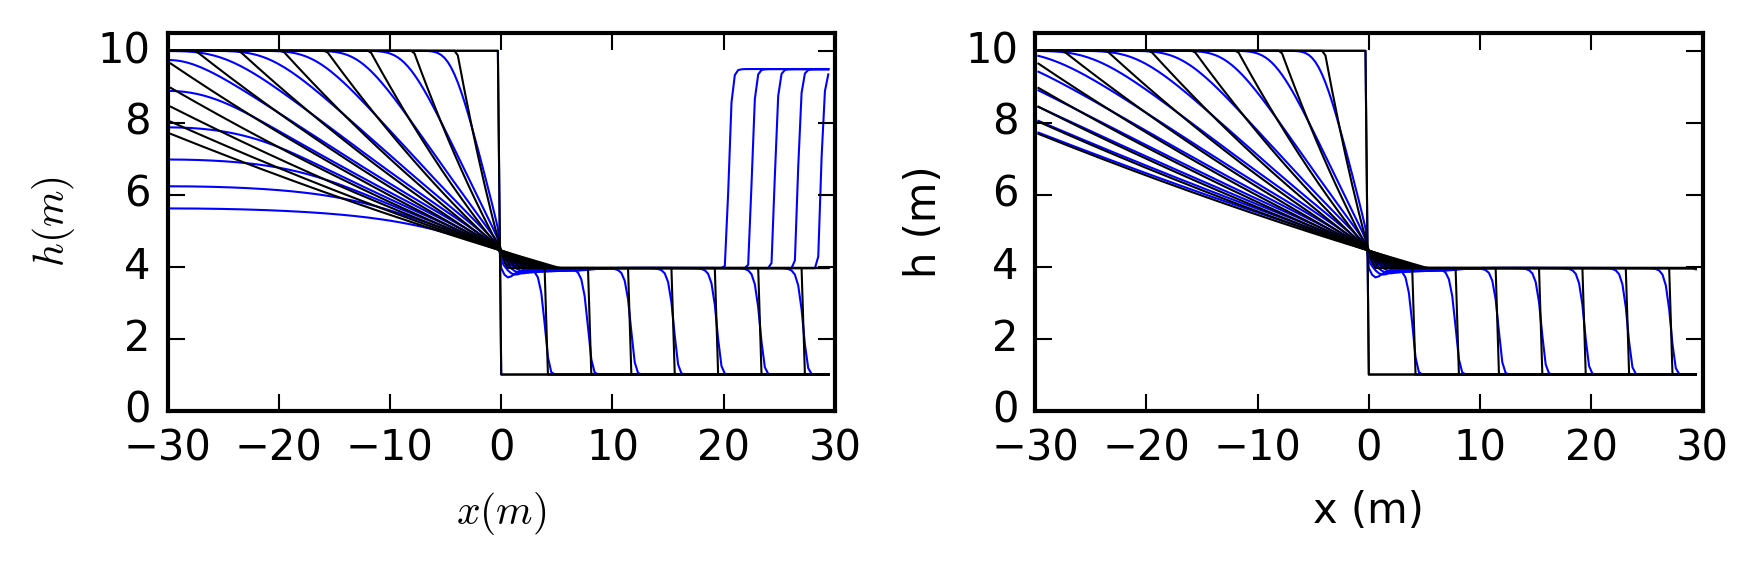
\includegraphics[width=\textwidth]{figures/db_hwet.png}


		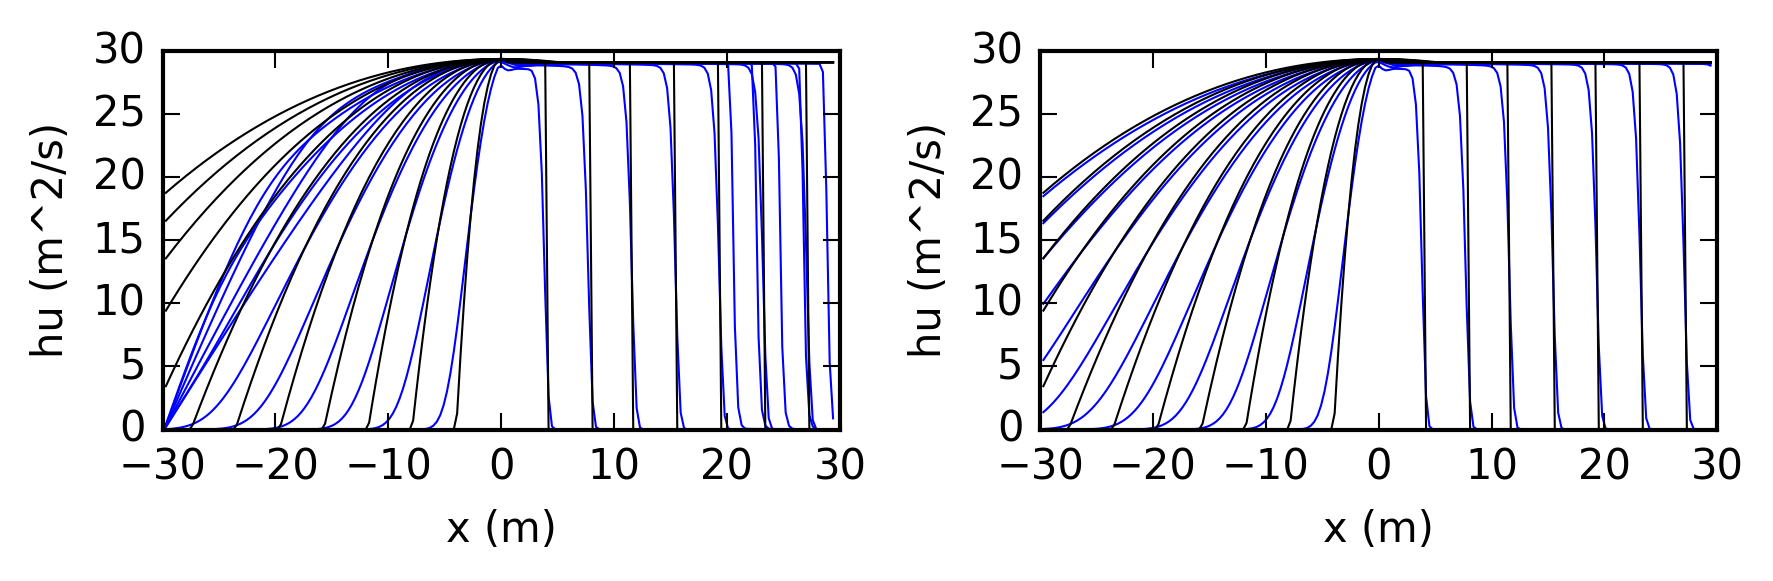
\includegraphics[width=\textwidth]{figures/db_huwet.png}
		\caption{Results for $h$ (top row) and $hu$ (bottom row) for the dambreak Case \#1 (wet-channel), using closed (left column) and open boundaries (right column). Blue line = numerical solution; Black line = analytical solution.}
		\label{nswe:wetchannel}
	\end{figure}
	\begin{figure}
		\centering
		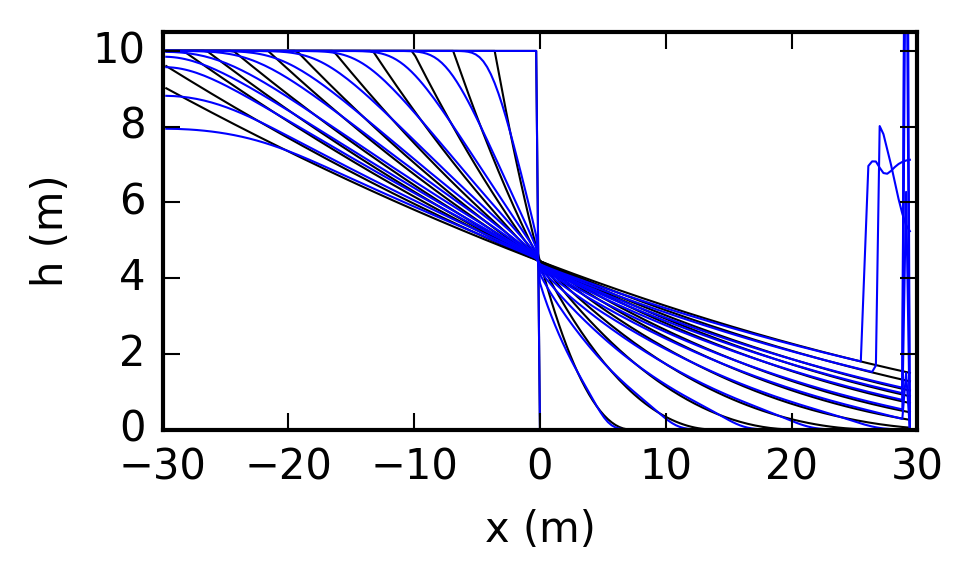
\includegraphics{figures/db_hdry.png}
		\caption{Results for $h$ for the dambreak Case \#6 (dry-$10^{-5}$ channel) using closed boundaries. Blue line = numerical solution; Black line = analytical solution}
		\label{nswe:drychannel}
	\end{figure}

	\begin{figure}
		\centering
		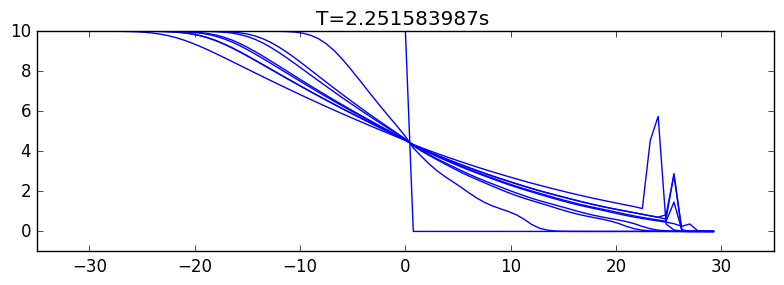
\includegraphics[width=0.8\textwidth]{figures/surfwb_1dfig000320.png}
		\caption{Results obtained for $h$ with SurfWB-UC for the dambreak Case \#8. Notice the bump propagating back from the right boundary. }
		\label{nswe:surfwb}
	\end{figure}

	\subsubsection{Second order scheme}

	Figure \ref{nswe:second_order} shows results for variable $h$ using the second order scheme using closed boundaries on the dry channel case. The left panel of the figure corresponds to the closed boundary conditions according to formulas of section \ref{nswe:bcs}. Results under these conditions showed negative water heights, which explains why the blue lines of the calculated results do not follow all the black lines of the analytical solution. However, a modified boundary condition was used,
	by just copying the same values in the second (farthest) ghost cells, whose results are shown in the right panel of figure \ref{nswe:second_order}, and did not show negative heights but only some small oscillations.

	\begin{figure}
		\centering
		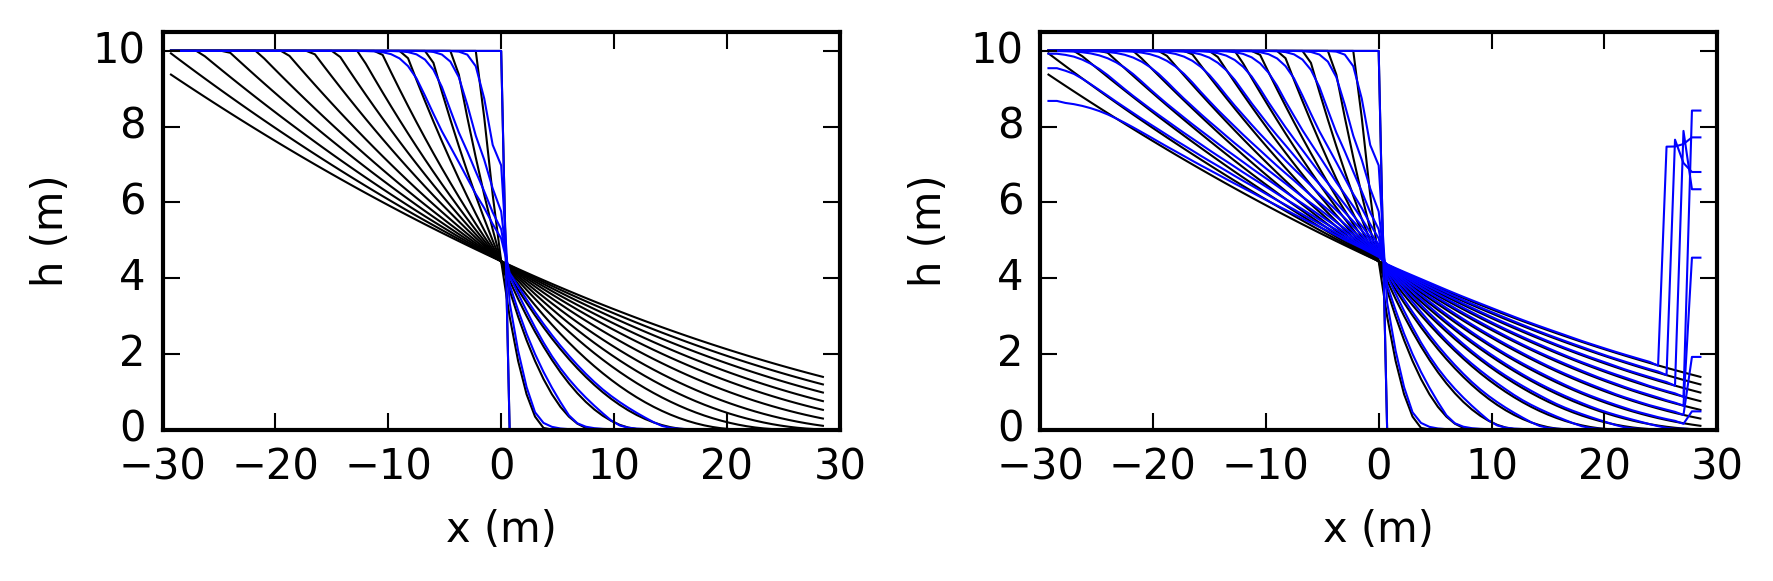
\includegraphics[width=\textwidth]{figures/db2_hdry.png}
		\caption{Results obtained for $h$ with the second order scheme using two kinds of closed boundaries. The boundary conditions explained in section \ref{nswe:bcs} (left) and the modified homogeneous Neumann boundary condition (right). }
		\label{nswe:second_order}
	\end{figure}

	\subsubsection{Fourth order scheme}

	Simulations were run using the fourth order scheme for both wet and dry channel cases. This time when using closed boundaries no negative depths were observed during the simulations. 	Also, results for the dambreak case using only open boundaries, for both dry and wet cases are shown in figure \ref{nswe:fourth_order}. Comparing these results with those of figure \ref{nswe:wetchannel} and \ref{nswe:drychannel} it can be observed that bigger differences and more dissipative-like effects appear compared to the lower order schemes, specially around the shock-wave, which can be observed in more mild slope in the front of the shock wave. 


	\begin{figure}[ht]
		\centering
		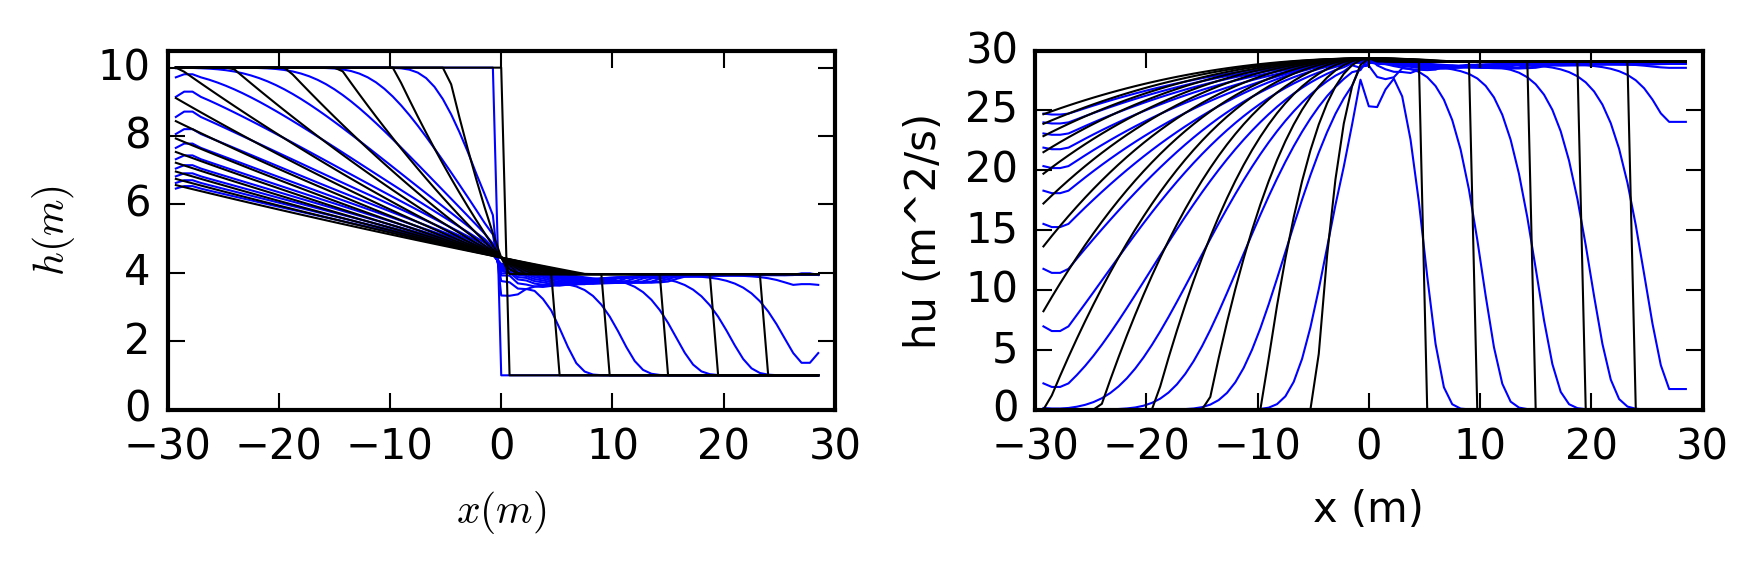
\includegraphics[width=\textwidth]{figures/db4_wet.png}

		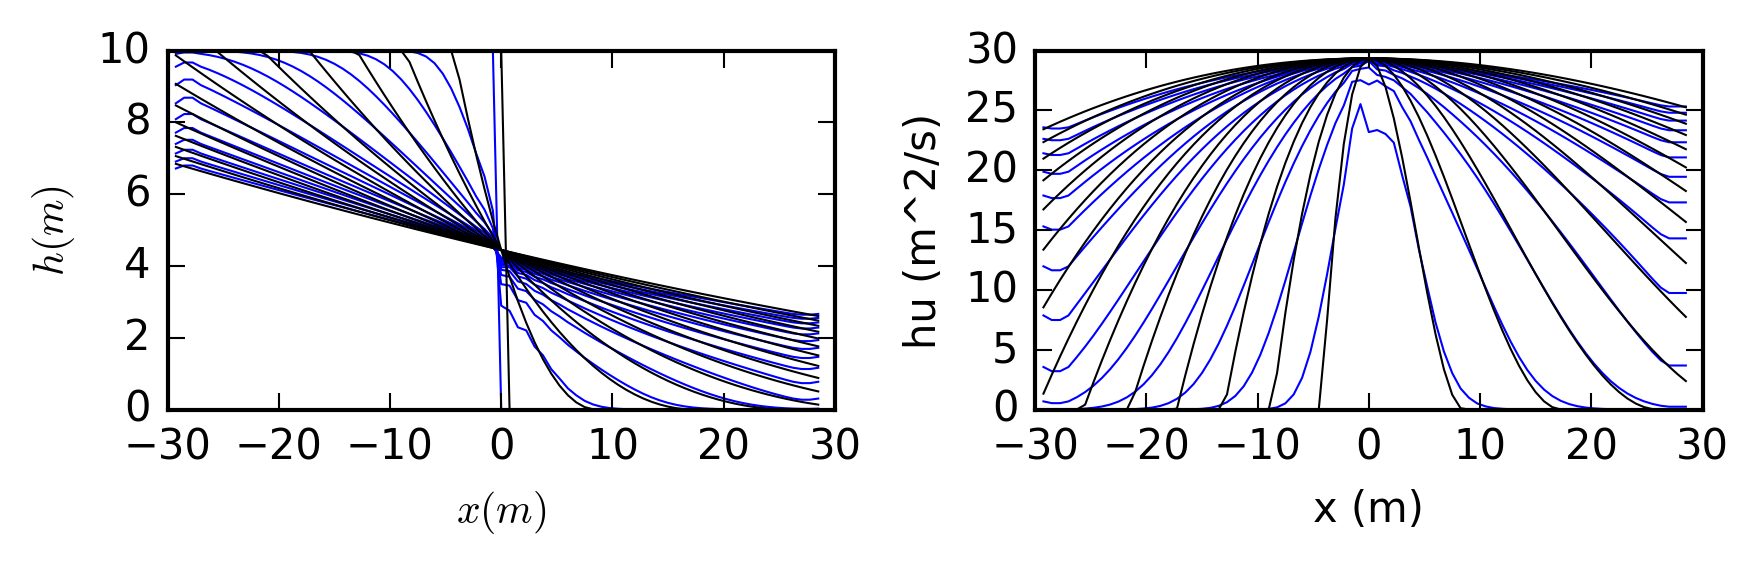
\includegraphics[width=\textwidth]{figures/db4_dry.png}
		\caption{Results obtained with the fourth order scheme for $h$ and $hu$ (left and right columns), for the initially wet or dry case (first and second row). }
		\label{nswe:fourth_order}
	\end{figure}

	\section{Remarks}

	Some important remarks of the work until this part are:
	\begin{itemize}
		\item Three numerical schemes of different order were implemented as discretization of the NSWE.
		\item Of them, the first and second order schemes were very sensitive to zero water depth when interacting with closed boundaries, showing numerical instabilities. The open boundaries did not show this issue.
		\item The fourth order scheme showed no trouble with vanishing depths when using open or closed boundary conditions. However, more dissipative effects are observed, specially around shock waves.
	\end{itemize}
